% --------------------------------------------------------------
% This is all preamble stuff that you don't have to worry about.
% Head down to where it says "Start here"
% --------------------------------------------------------------

\documentclass[12pt]{article}

\usepackage[margin=1in]{geometry}
\usepackage{amsmath,amsthm,amssymb}
\usepackage{graphicx}
\usepackage{listings}

\newcommand{\N}{\mathbb{N}}
\newcommand{\Z}{\mathbb{Z}}

\newenvironment{theorem}[2][Theorem]{\begin{trivlist}
\item[\hskip \labelsep {\bfseries #1}\hskip \labelsep {\bfseries #2.}]}{\end{trivlist}}
\newenvironment{lemma}[2][Lemma]{\begin{trivlist}
\item[\hskip \labelsep {\bfseries #1}\hskip \labelsep {\bfseries #2.}]}{\end{trivlist}}
\newenvironment{exercise}[2][Exercise]{\begin{trivlist}
\item[\hskip \labelsep {\bfseries #1}\hskip \labelsep {\bfseries #2.}]}{\end{trivlist}}
\newenvironment{problem}[2][Problem]{\begin{trivlist}
\item[\hskip \labelsep {\bfseries #1}\hskip \labelsep {\bfseries #2.}]}{\end{trivlist}}
\newenvironment{question}[2][Question]{\begin{trivlist}
\item[\hskip \labelsep {\bfseries #1}\hskip \labelsep {\bfseries #2.}]}{\end{trivlist}}
\newenvironment{corollary}[2][Corollary]{\begin{trivlist}
\item[\hskip \labelsep {\bfseries #1}\hskip \labelsep {\bfseries #2.}]}{\end{trivlist}}

\newtheorem*{claim}{Claim}


\begin{document}

% --------------------------------------------------------------
%                         Start here
% --------------------------------------------------------------

\title{Homework 1}%replace X with the appropriate number
\author{Erich Menge (menge053) \\ %replace with your name
Algorithms \& Data Structures Section 003} %if necessary, replace with your course title

\maketitle

\begin{problem}{6.1-1} What are the minimum and maximum numbers of elements in a heap of height $h$? \\

    The height of a tree is the number of edges on the longest path from the root to a leaf. If we take a complete binary tree
    in which all leaves are of the same height and all parents have two children, and add one node to the very left, we will have
    a tree with $\boxed{2^{h}}$ nodes. So this is the minimum number of nodes we can have in a tree of $h$ height.

    Using this same logic, we can fill this entire layer by letting the number of nodes equal $2^{h+1}$. But now we
    have an extra node, which must be subtracted. So the maximum number of nodes in a tree of height $h$ is $\boxed{2^{h+1} - 1}$.
    \begin{figure}[h!]
        \centering
        \caption{Tree of height $h$}
        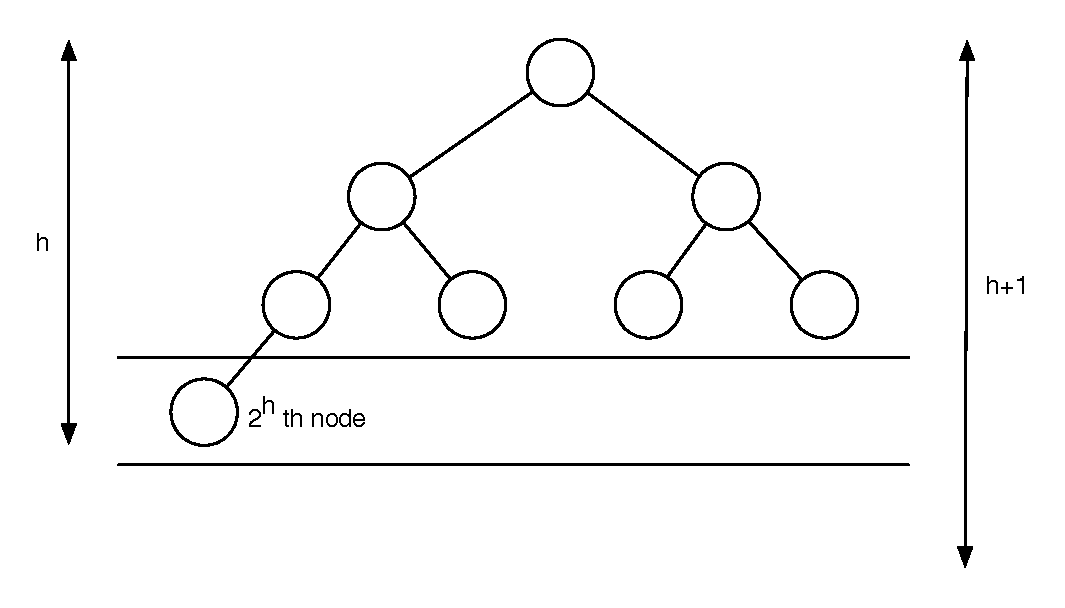
\includegraphics[scale=.75]{bin_tree1.eps}
        \label{fig:bintree1}
    \end{figure}
\end{problem}

\newpage
\begin{problem}{6.1-2} Show that an $n$-element heap has height $\lfloor \lg n \rfloor$ \\
  \claim $h = \lfloor \lg n \rfloor$
  \begin{proof}
    \begin{alignat*}{4}
      2^{h} &\le n &<& 2^{h+1} \text{ (demonstrated in Problem 6.1.1)} \\
      h &\le \lg n &<& h+1
    \end{alignat*}
    $\lg n < h + 1$ and $\lg n \ge h$ so $\lg n = h$. But $h \in \Z$, so $h = \lfloor \lg n \rfloor$. We take
    the floor because $h$ must be an integer, and rounding up would make $h$ too large by definition $\lg n < h + 1$.
  \end{proof}
\end{problem}

\begin{problem}{6.1-7} Show that, with the array representation for storing an $n$-element heap, the leaves are the nodes indexed
  by $\lfloor n/2 \rfloor + 1$, $\lfloor n/2 \rfloor + 2$, $\ldots$,$n$.
  \begin{proof}\ \\

    \noindent{\bf Basis:}

    Let $n = 1$ for a heap with 1 node.
    Because there is only one node, it must be a leaf. $\lfloor (1)/2 \rfloor + 1 = 1\checkmark$. \\

    \noindent{\bf Inductive Step:}

     Each parent can have at most $2$ leaves. We are dividing by two and taking the floor, so the function increases on even numbers of nodes.
     When we add a node its parent is the first leaf in the heap. Adding the child means the parent is no longer a leaf. A single child also means that there is now an even
     number of nodes so the function increases by one. If another child is added to the parent it will not increase the function
     and the index of the first leaf remains the same because there is now an odd number of nodes. This demonstrates $\lfloor n/2 \rfloor + 1$ is always the index of the first leaf.

     Since all children are added to the last leaf, all nodes between the first leaf and $n$ must also be leaves.
  \end{proof}
\end{problem} \newpage

\begin{problem}{6.2-5} Rewrite MAX-HEAPIFY with iteration. \\
\begin{figure}[h!]
  \centering
  \caption{Original Listing}
  \begin{lstlisting}
    MAX-HEAPIFY(A, i)
      l = LEFT(i)
      r = RIGHT(i)
      if l <= A.heap-size and A[l] > A[i]
        largest = l
      else largest = i
      if r <= A.heap-size and A[r] > A[largest]
        largest = r
      if largest != i
        exchange A[i] with A[largest]
        MAX-HEAPIFY(A, largest)
  \end{lstlisting}
  \label{fig:listing1}
\end{figure}

\begin{figure}[h!]
  \centering
  \caption{Listing \ref{fig:listing1} with an Iterative Loop}
  \begin{lstlisting}
    MAX-HEAPIFY(A, i)
      l = LEFT(i)
      r = RIGHT(i)

      if l <= A.heap-size and A[l] > A[i]
        largest = l
      else largest = i
      if r <= A.heap-size and A[r] > A[largest]
        largest = r

      while largest != i do
        exchange A[i] with A[largest]
        i = largest

        l = LEFT(i)
        r = RIGHT(i)

        if l <= A.heap-size and A[l] > A[i]
          largest = l
        else largest = i
        if r <= A.heap-size and A[r] > A[largest]
          largest = r
      end

  \end{lstlisting}
\end{figure}
\end{problem} \newpage

\begin{problem}{6.3-3} Show that there are at most $\lceil n/2^{h+1} \rceil$ nodes of height h in any n-element heap. \\
  \begin{proof}\ \\

  \noindent {\bf Basis Step:} \\

  \indent Let $h = 0$ in a heap of height $2$ (see figure \ref{fig:bintree2}). \\
  \indent Then $4 \le \lceil 7/2^{0+1} \rceil = 4 \checkmark$ \\

  \noindent {\bf Inductive Step:} \\

  We know from problem 6.1-2 that the first leaf is indexed by $\lfloor n/2 \rfloor + 1$. So that means the last parent must
  be indexed by $\lfloor n/2 \rfloor$. The index of the last parent is also the number of parents in the heap. So
  $n - \lfloor n/2 \rfloor$ or $\lceil n/2 \rceil$ is the number of leaves in a heap. So we can then take a heap of height $h - 1$
  to have $n - \lceil n/2 \rceil$ or $\lfloor n/2 \rfloor$ nodes. Using the given function we have the number of nodes at $h - 1$
  given by $\lceil n/2^{h+1-1} \rceil = \lceil n/2^{h} \rceil$. Using $n - \lceil n/2 \rceil$ or $\lfloor n/2 \rfloor$ as our
  value of $n$ in the $h - 1$ tree we have:
  \begin{align*}
    \lceil (\lfloor n/2 \rfloor)/2^{h} \rceil &\le \lceil n/2^{h+1} \rceil \\
    \lceil 2^{-h} \cdot \lfloor n/2 \rfloor \rceil &\le  \lceil n \cdot 2^{-h-1} \rceil \\
    \lceil 2^{-h} \cdot \lfloor n/2 \rfloor \rceil &\le  \lceil n \cdot 2^{-h}\cdot 2^{-1} \cdot \rceil \\
    \lceil \lfloor n/2 \rfloor \rceil &\le  \lceil (1/2)n\rceil \\
    n &= n
  \end{align*}
  This shows that the given function works works on all sub-heaps of a heap of height $h$.
  \end{proof}
  \begin{figure}[!h]
    \centering
    \caption{Binary Tree of height $h$}
    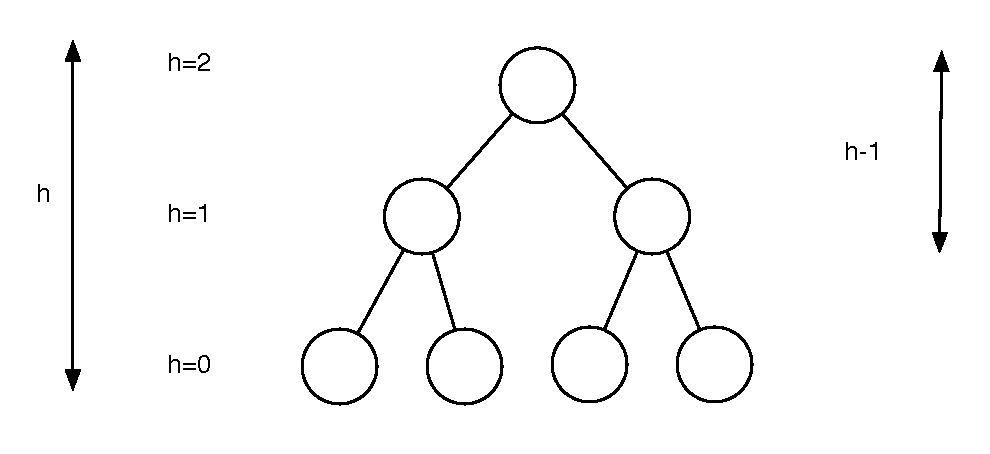
\includegraphics[scale=.75]{bin_tree2.eps}
    \label{fig:bintree2}
  \end{figure}
\end{problem}

% --------------------------------------------------------------
%     You don't have to mess with anything below this line.
% --------------------------------------------------------------

\end{document}